\section{DSP}

\begin{frame}{Inlets para DSP}
\begin{figure}[h!]
\centering
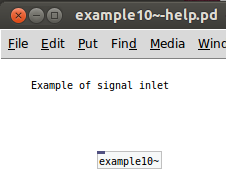
\includegraphics[width=0.5\textwidth]{example10}
\caption{Primeiro Inlet DSP}
\end{figure}
\end{frame}


\begin{frame}{Inlets para DSP}
Alguns pontos importantes:
\begin{itemize}
\item Existem macros para facilitar a definição do primeiro inlet para classes
do tipo \texttt{CLASS\_DEFAULT}.
\item Inlets adicionais são instanciados no método \texttt{\_new()}.
\end{itemize}
\end{frame}


\begin{frame}[fragile]{Código para o primeiro inlet DSP (1/2)}
{Estrutura e métodos \texttt{\_perform()} e \texttt{\_dsp()}}

\begin{lstlisting}
typedef struct _example10 {
    t_object x_obj;
    t_float x_f; /* inlet value when set by message */
} t_example10;

static t_int * example10_perform(t_int *w){
  t_float     *in = (t_float *) (w[1]);
  int          n  = (int) (w[2]);
  t_example10 *x  = (t_example10 *) (w[3]);
  // do something ...
  return (w + 4); // next block's address
}

static void example10_dsp(
         t_example10 *x, t_signal **sp){
  // adds a method for dsp
  dsp_add(example10_perform, 3, sp[0]->s_vec, sp[0]->s_n, x);
}
\end{lstlisting}

\end{frame}


\begin{frame}[fragile]{Código para o primeiro inlet DSP (2/2)}
{Método \texttt{\_setup()}}
\begin{lstlisting}
void example10_tilde_setup(void) {
  example10_class = class_new(gensym("example10~"),
    (t_newmethod) example10_new, // Constructor
    (t_method) example10_destroy, // Destructor
    sizeof (t_example10),
    CLASS_DEFAULT,
    A_GIMME,
    0);
  // this declares the leftmost, "main" inlet
  // as taking signals.
   CLASS_MAINSIGNALIN(example10_class, t_example10, x_f);
   class_addmethod(example10_class, (t_method) example10_dsp, gensym("dsp"), 0);
}
\end{lstlisting}

\end{frame}


\begin{frame}{Inlets DSP adicionais (1/3)}
\begin{figure}[h!]
\centering
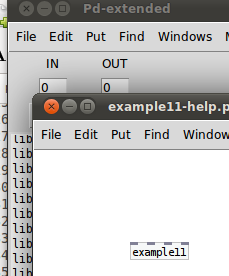
\includegraphics[width=0.3\textwidth]{example11}
\end{figure}
\end{frame}


\begin{frame}[fragile]{Inlets DSP adicionais (2/3)}
{Método \texttt{\_new()}}
\begin{lstlisting}
// Constructor of the class
void * example11_new(t_symbol *s, int argc, t_atom * argv) {
    t_example11 *x = (t_example11 *) pd_new(example11_class);
    inlet_new(&x->x_obj, &x->x_obj.ob_pd, &s_signal, &s_signal); // second signal inlet
    inlet_new(&x->x_obj, &x->x_obj.ob_pd, &s_signal, &s_signal); // third signal inlet
    inlet_new(&x->x_obj, &x->x_obj.ob_pd, &s_signal, &s_signal); // fourth signal inlet
    return (void *) x;
}
\end{lstlisting}
\end{frame}


\begin{frame}[fragile]{Inlets DSP adicionais (3/3)}
{Métodos \texttt{\_perform()} e \texttt{\_dsp()}}
\begin{lstlisting}
static t_int * example11_perform(t_int *w){
  t_float *in1 = (t_float *)(w[1]);
  t_float *in2 = (t_float *)(w[2]);
  t_float *in3 = (t_float *)(w[3]);
  t_float *in4 = (t_float *)(w[4]);
  int n = (int)(w[5]);
  t_example11 *x = (t_example11 *)(w[6]);
  return (w + 7); // proximo bloco
}

static void example11_dsp(
      t_example11 *x, t_signal **sp){
  dsp_add(example11_perform, 6, sp[0]->s_vec, sp[1]->s_vec, sp[2]->s_vec, sp[3]->s_vec, sp[0]->s_n, x);
}
\end{lstlisting}
\end{frame}


\begin{frame}{Outlets DSP (1/2)}
\begin{figure}[h!]
\centering
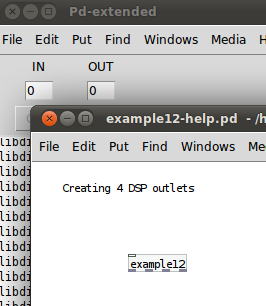
\includegraphics[width=0.3\textwidth]{example12}
\end{figure}
\end{frame}


\begin{frame}[fragile]{Outlets DSP (2/2)}{Método \texttt{\_new()}}
\begin{lstlisting}
typedef struct _example12 {
   t_object x_obj;
   t_outlet * x_outlet_dsp_0;
   t_outlet * x_outlet_dsp_1;
   t_outlet * x_outlet_dsp_2;
   t_outlet * x_outlet_dsp_3;

} t_example12;

void * example12_new(void){
   t_example12 *x = (t_example12 *) pd_new(example12_class);
   x->x_outlet_dsp_0 = outlet_new(&x->x_obj, &s_signal);
   x->x_outlet_dsp_1 = outlet_new(&x->x_obj, &s_signal);
   x->x_outlet_dsp_2 = outlet_new(&x->x_obj, &s_signal);
   x->x_outlet_dsp_3 = outlet_new(&x->x_obj, &s_signal);
   return (void *) x;
}

\end{lstlisting}
\end{frame}


\begin{frame}{Inlets e outlets criados dinamicamente (1/4)}
\textbf{Cenário:} o objeto possui um número de inlets (e outlets) igual a um parâmetro
passado no momento de sua criação. 
\end{frame}


\begin{frame}[fragile]{Inlets e outlets criados dinamicamente (2/4)}
{Estrutura e método \texttt{\_dsp()}}
\begin{lstlisting}
typedef struct _multigain {
   t_object x_obj;
   t_int count;
   t_float gain;
   t_inlet * x_inlet_gain_float;
   t_sample ** invec;
   t_sample ** outvec;
} t_multigain;
static void multigain_dsp(t_multigain *x, t_signal **sp){
   if(x->count < 1) return;
   int i = 0;
   for(; i < x->count; i++){
      x->invec[i] = getbytes(sys_getblksize() * sizeof(t_sample));
      x->invec[i] = sp[i]->s_vec;
      x->outvec[i] = getbytes(sys_getblksize() * sizeof(t_sample));
      x->outvec[i] = sp[x->count + i]->s_vec;
   }
   dsp_add(multigain_perform, 2, x, sp[0]->s_n);
}

\end{lstlisting}
\end{frame}


\begin{frame}[fragile]{Inlets e outlets criados dinamicamente (3/4)}
{Método \texttt{\_new()}}
\begin{lstlisting}
void * multigain_new(t_floatarg count_arg){
   t_multigain *x = (t_multigain *) pd_new(multigain_class);
   x->count = (int)count_arg;
   short i;
   for (i = 0; i < x->count; i++) {
      inlet_new(&x->x_obj, &x->x_obj.ob_pd, &s_signal, &s_signal); // signal inlets
      outlet_new(&x->x_obj, &s_signal);
   }
   x->outvec = getbytes(sizeof(t_sample) * x->count);
   x->invec = getbytes(sizeof(t_sample) * x->count);
   x->x_inlet_gain_float = floatinlet_new(&x->x_obj, &x->gain);
   return (void *) x;
}
\end{lstlisting}
\end{frame}


\begin{frame}[fragile]{Inlets e outlets criados dinamicamente (4/4)}
{Método \texttt{\_perform()}}
\begin{lstlisting}
static t_int * multigain_perform(t_int *w){
   t_multigain *x = (t_multigain *)(w[1]);
   int n = (int)(w[2]), i = 0, j = 0;
   float gain = x->gain;
   for(; i < x->count ; i++)
      for(j = 0 ; j < n ; j++)
         x->outvec[i][j] = x->invec[i][j] * gain;
   return (w + 3); // proximo bloco
}
\end{lstlisting}
\end{frame}
